\documentclass[a4paper]{scrartcl}
\usepackage[cm]{fullpage}
\usepackage{amsmath, amssymb, esint}
\usepackage{siunitx}
\usepackage[space]{grffile}

\usepackage{tikz, pgfplots}
\pgfplotsset{
    compat = 1.12,
    plot-scatter/.style = {
        only marks,
        error bars/.cd,
        x dir = both, y dir = both,
        x explicit, y explicit
    }
}

\begin{document}

\title{PHYS3112: Properties of Laser Light}
\author{ \\ \\ }
\date{2017-04-10}
\maketitle

\begin{abstract}
    Various properties of HeNe laser light are observed and compared to the theory, including its spectrum, beam divergence, stability and coherence. They match, as one would hope.
\end{abstract}

\section{Materials and Methods}
Please refer to the operating instructions of the experiment.

\section{Results}
\subsection{Experiment 1: Wavelength of Red Light}
Using a diffraction grating of 16000 lines per inch (or \SI{1.59}{\micro\metre} line spacing), the 1st-to-1st order maxima distance was \SI{80 \pm 1}{\milli\metre} at a perpendicular distance of \SI{92.5 \pm 0.5}{\milli\metre} from the grating. This corresponds to a wavelength of \SI{630 \pm 7}{\nano\metre}.

\subsection{Experiment 2: Spectroscopy}
\begin{figure}
    \centering
    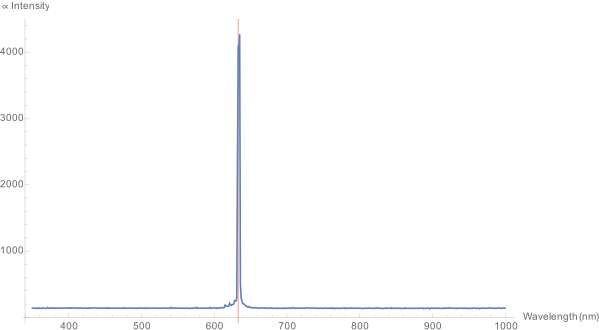
\includegraphics[height = 10cm]{Q2/HeNe Laser.png}
    \caption{HeNe Laser Spectrum}
    \label{fig:hene-laser}
\end{figure}
\begin{figure}
    \centering
    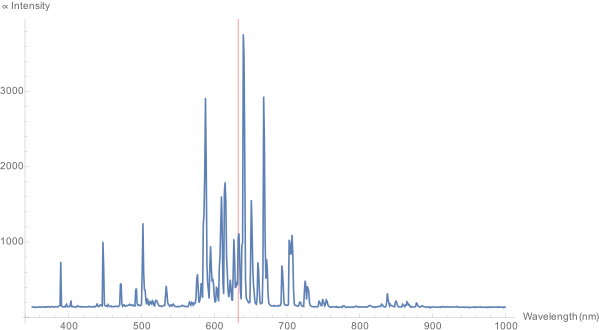
\includegraphics[height = 10cm]{Q2/HeNe Cavity.png}
    \caption{HeNe Cavity Spectrum}
    \label{fig:hene-cavity}
\end{figure}
\begin{figure}
    \centering
    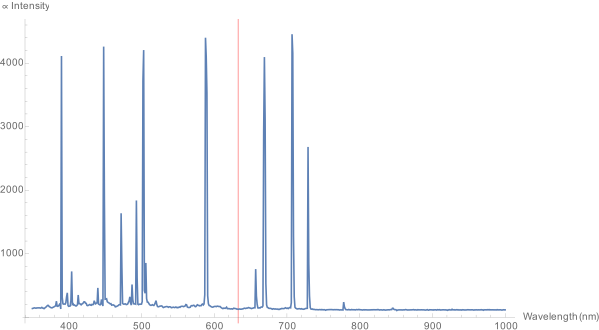
\includegraphics[height = 10cm]{Q2/Helium Plasma.png}
    \caption{Helium Plasma Spectrum}
    \label{fig:he-plasma}
\end{figure}
\begin{figure}
    \centering
    \includegraphics[height = 10cm]{Q2/Neon Plasma.png}
    \caption{Neon Plasma Spectrum}
    \label{fig:ne-plasma}
\end{figure}
\begin{figure}
    \centering
    \includegraphics[height = 10cm]{Q2/Incandescent.png}
    \caption{Incandescent Bulb Spectrum}
    \label{fig:incandescent}
\end{figure}
\begin{figure}
    \centering
    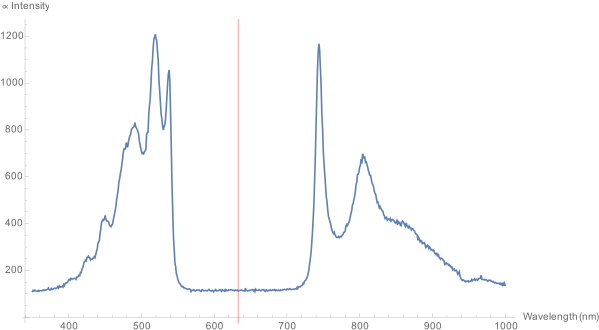
\includegraphics[height = 10cm]{Q2/Incandescent + Cavity.png}
    \caption{Incandescent Bulb Spectrum when viewed through a HeNe laser cavity}
    \label{fig:incandescent-cavity}
\end{figure}

Figure \ref{fig:hene-laser} shows the output of the laser itself, with clear sharp peak around \SI{635}{\nano\metre}. In the cavity spectrum in Figure \ref{fig:hene-cavity}, however, the \SI{635}{\nano\metre} line is only a minor peak, with it surrounded by much larger peaks.

Both the helium and neon plasmas in Figures \ref{fig:he-plasma} and \ref{fig:ne-plasma} have numerous peaks, of which the largest 5 are at around 390, 448, 503, 588 and \SI{707}{\nano\metre} for helium, and 611, 616, 635, 642 and \SI{652}{\nano\metre} for neon.

The incandescent bulb spectrum in Figure \ref{fig:incandescent} shows a shape similar to that of a black body radiator, but with a ripple added on top, while the same spectrum passed through a HeNe laser cavity in Figure \ref{fig:incandescent-cavity} has a large trough around the \SI{633}{\nano\metre} lasing frequency.

\subsection{Experiment 3: Beam Divergence}
\begin{figure}
    \centering
    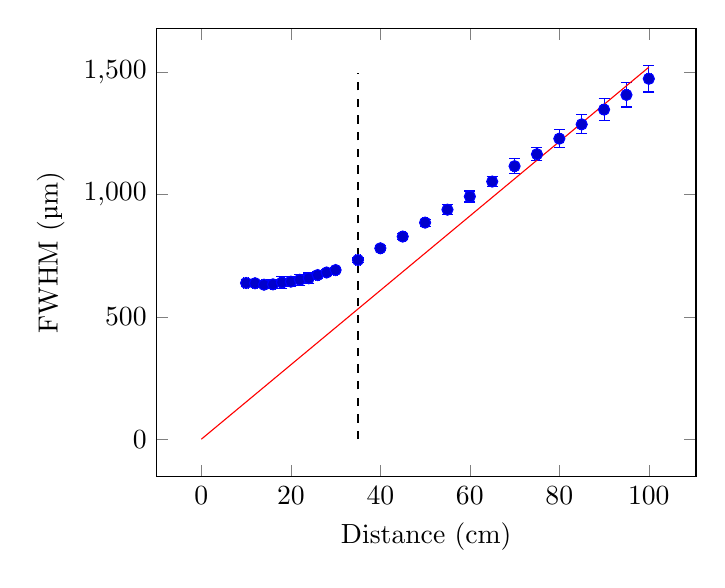
\begin{tikzpicture}
        \begin{axis}[
            xlabel = Distance (\si{\centi\metre}),
            ylabel = FWHM (\si{\micro\metre})
        ]
            \addplot +[plot-scatter] table [
                x error = xerror,
                y error = yerror
            ] {
                x       y       xerror  yerror
                10.0	639.0	0.5	14.5
                12.0	638.0	0.5	8.5
                14.0	632.0	0.5	11.0
                16.0	633.5	0.5	18.0
                18.0	641.0	0.5	24.0
                20.0	644.5	0.5	21.0
                22.0	652.0	0.5	21.5
                24.0	658.5	0.5	21.5
                26.0	671.5	0.5	15.0
                28.0	682.0	0.5	13.0
                30.0	692.0	0.5	9.0
                35.0	733.0	0.5	8.5
                40.0	781.0	0.5	10.0
                45.0	829.0	0.5	11.5
                50.0	886.0	0.5	14.5
                55.0	939.0	0.5	20.5
                60.0	993.0	0.5	22.5
                65.0	1054.0	0.5	20.0
                70.0	1117.0	0.5	31.5
                75.0	1166.0	0.5	26.5
                80.0	1229.5	0.5	36.0
                85.0	1288.0	0.5	39.0
                90.0	1348.5	0.5	46.0
                95.0	1408.5	0.5	49.5
                100.0	1474.5	0.5	54.0
            };
            \addplot +[no marks, domain = 0:100] {15.2182 * x};
            \draw [dashed] (35, 0) -- (35, 1500);
        \end{axis}
    \end{tikzpicture}
    \caption{FWHM of the beam versus distance}
    \label{fig:beam-divergence}
\end{figure}

Our beam width measurements can be seen in Figure \ref{fig:beam-divergence}. Due to the beam cross section not being perfectly circular, both major and minor axes FWHM measurements were taken (and their errors from fitting a gaussian), and then combined by taking a weighted mean. The error is simply half the maximum width minus the minimum width.

To find the net beam divergence, we simply fit a line starting at the origin to the measurements far from the aperture (say, at least \SI{60}{\centi\metre} away), and convert the gradient to an angle. There are better asymptote finding methods, but this is sufficient enough for our purposes, and produces a result of \SI{1.52 \pm 0.27}{\milli\radian}.

This corresponds to a beam waist of \SI{0.26 \pm 0.05}{\milli\metre} and a Rayleigh range of \SI{35 \pm 12}{\centi\metre}.

\subsection{Experiment 4: Spatial Filter}
While data was collected for this experiment, it turned out we had our filter the wrong way around (with the lens after the pinhole), and hence makes the results invalid. As such, this experiment will be skipped.

\subsection{Experiment 5: Granularity of Scattered Light}
\begin{table}
    \centering
    \begin{tabular}{c | c}
        Lens & Speckle vs Head Movement \\
        \hline
        None & Opposite \\
        Yellow & Same \\
        Red & Opposite \\
        Blue & Opposite \\
        Green & Opposite \\
        Brass & Same
    \end{tabular}
    \caption{Direction of movement of the laser speckles due to head movement}
    \label{tab:speckles}
\end{table}
Our results for this experiment can be seen in Table \ref{tab:speckles}. "Same" means the speckles moved in the same direction as the head (i.e., opposite to the movement of the background), while "Opposite" means the opposite. None of the measurements produced speckles that were stationary with respect to the background.

\subsection{Experiment 6: Laser Stability}
\begin{figure}
    \centering
    \includegraphics[width = 18cm]{Q6/plot.png}
    \caption{Intensity of the laser during warm up}
    \label{fig:warm-up}
\end{figure}
The intensity of the laser during warm up can be seen in Figure \ref{fig:warm-up}. The momentary dips in intensity correspond to accidentally blocking the laser beam, and should be ignore. Notably, one can see oscillations of different frequencies in the intensity, with the oscillations most pronounced with the polarising filter.

\subsection{Experiment 7: Longitudinal Modes}
This experiment was accidentally skipped during the lab, so there are no results to be shown here.

\subsection{Experiment 8: Beam Coherence}
\subsubsection{Spatial Coherence}
The beam was observed to show interference patterns across its entire cross section, with minima that matches the background levels (according to the naked eye).

\subsubsection{Temporal Coherence}
\begin{figure}
    \centering
    \includegraphics[width = 18cm]{Q8/plot.png}
    \caption{Interference visibility given a path difference}
    \label{fig:interference-visibility}
\end{figure}
The interference visibility with different path length differences can be seen in Figure \ref{fig:interference-visibility}. There is a clear maxima around a path difference of 0, while the visibility approaches a minima as the path difference towards the tail of our plot. This would put our coherence length to around \SI{30 \pm 5}{\centi\metre}, or \SI{1.0 \pm 0.2}{\nano\second}.

\section{Discussion}
\subsection{Experiment 1: Wavelength of Red Light}
Our experimental value of \SI{630 \pm 7}{\nano\metre} agrees with the value of \SI{633}{\nano\metre} quoted for the laser.

\subsection{Experiment 2: Spectroscopy}
\begin{table}
    \centering
    \begin{tabular}{c | c | c}
        \(\lambda\) \si{\nano\metre} & Upper level & Lower level \\
        \hline
        389 & 3p & 2s \\
        447 & 4d & 2p \\
        502 & 3p & 2s \\
        588 & 3d & 2p \\
        707 & 3s & 2p
    \end{tabular}
    \caption{Certain helium spectral lines with their corresponding transitions}
    \label{tab:helium-lines}
\end{table}
\begin{table}
    \centering
    \begin{tabular}{c | c | c}
        \(\lambda\) \si{\nano\metre} & Upper level & Lower level \\
        \hline
        607 & 3p & 3s \\
        616 & 3p & 3s \\
        633 & 3p & 3s \\
        640 & 3p & 3s \\
        651 & 3p & 3s
    \end{tabular}
    \caption{Certain neon spectral lines with their corresponding transitions}
    \label{tab:neon-lines}
\end{table}
The peak observed in the laser output is slightly offset from the quoted value of \SI{633}{\nano\metre} by \SI{2}{\nano\metre}. This might simply be due to a resolution or calibration issue with the spectroscope.

The peaks seen in the HeNe cavity matches quite well to the combination of the helium and neon plasma spectra, though the relative intensities seem to differ fairly significantly.

Meanwhile, for the helium and neon plasma, the NIST ASD quotes the values in Tables \ref{tab:helium-lines} and \ref{tab:neon-lines}, and they agree with our five largest peaks to within \SI{2}{\nano\metre}. One thing to note is that neon has a line at \SI{633.4}{\nano\metre} that is about three times more intense than the line at \SI{632.8}{\nano\metre} used for lasing.

\subsection{Experiment 3: Beam Divergence}
With the quoted \SI{0.88}{\milli\metre} beam aperture for this laser (which we assume to be the \(\frac{1}{e^2}\) value), converting it to FWHM and halving it produces a beam waist of \SI{0.26}{\milli\metre}. This agrees with our experimental results.

Such a beam waist allows an optimal beam divergence of \SI{1.55}{\milli\radian}, which matches our observed beam divergence, and hence we can say our laser is diffraction limited in beam divergence.

\subsection{Experiment 5: Granularity of Scattered Light}
When the speckles move in the same direction as the head, it means the image was focused behind the retina (hyperopia); and moving the opposite direction indicates myopia. This agrees with the lenses used (except the yellow lens), as well as the fact that I am slightly myopic.

\subsection{Experiment 6: Laser Stability}
The highest frequency oscillations in the intensity are most likely due to mode sweeping, where different longitudinal modes ``sweep'' across the gain curve as the lasing cavity length changes due to thermal expansion. Since the total intensity is the sum of all the longitudinal mode intensities multiplied by the gain curve, the relative positions of the modes to the gain curve would affect the total intensity. The oscillation comes from the fact that there are numerous longitudinal modes permitted by the cavity, all spaced approximately evenly (about \SI{1.2}{\giga\hertz} with a \SI{25}{\centi\metre} long cavity and \SI{633}{\nano\metre} light), slowly ``entering'' the gain curve, moving through its maximum, and then ``exiting''.

This effect is even more apparent with the polarising filter, since mode sweeping also sweeps through the two orthogonal linear polarisation modes. This effect is maximised when the polariser is equal to one of the polarisation angles of the laser, and minimised when it is \SI{45}{\degree} to both, as one would expect. This can be seen in our measurements as the \SI{90}{\degree} ``peak-to-peak'' variance in output intensity with the polariser.

The lowest frequency oscillation seen, however, is of unknown origin, and might be due to fluctuations in the power supply.

\subsection{Experiment 8: Beam Coherence}
\subsubsection{Spatial Coherence}
The fact that the beam shows an interference pattern with intensity minima that goes to 0 indicates the beam is spatially coherent. In fact, any interferometry experiment with such minima would be indicative of spatial coherency.

\subsubsection{Temporal Coherence}
A \SI{30 \pm 5}{\centi\metre} coherence length is quite typical of off-the-shelf lasers. This coherence length corresponds to a line width of approximately \SI{1.0 \pm 0.2}{\giga\hertz}, indicative of a multimode laser.

If instead we had a single mode laser with a linewidth of \SI{1}{\mega\hertz}, we would have expected a coherence length of around \SI{300}{\metre}.

\end{document}